\Testart{Skript}
\Klasse{09}
\Fach{Informatik}
\Titel{Objektorientierte Programmierung mit Java (2)}

\renewcommand{\Content}{
    
    \mysession{Stunde 6+7}{

        \section{Taschenrechner}

\flushleft

\begin{minipage}{0.49\textwidth}
Implementiere das Klassendiagramm rechts mit Hilfe von Blockly. Probiere deine Methode aus (siehe Anleitung auf der Vorderseite). Fülle die Lücken im Java-Code unten aus, wenn deine Methoden funktionieren.
\end{minipage}
\hfill
\begin{minipage}{0.49\textwidth}
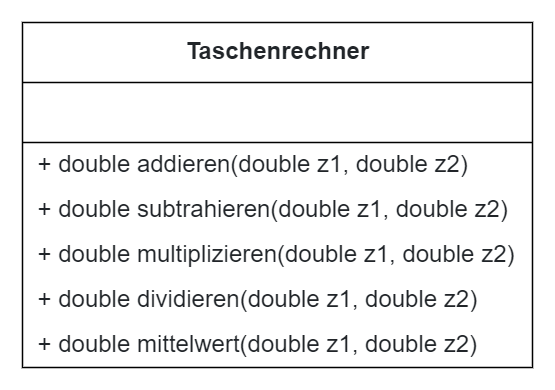
\includegraphics[width=\linewidth]{_Aufgaben/BlocksAndJava/img/Taschenrechner.png}
\end{minipage}

\LARGE


\begin{lstlisting}[escapechar=\&]

public class Taschenrechner
{    
    public & \LoesungLuecke{double addieren(double z1, double z2) \{ }{12cm} &
        
            & \LoesungLuecke{return z1 + z2;}{12cm} &
    }
    public &\LoesungLuecke{double subtrahieren(double z1, double z2) \{ }{12cm}&
        
            & \LoesungLuecke{return z1 - z2;}{12cm} &
    }
    public &\LoesungLuecke{double multiplizieren(double z1, double z2) \{ }{12cm}&
        
            & \LoesungLuecke{return z1 * z2;}{12cm} &
    }
    public & \LoesungLuecke{double dividieren(double z1, double z2) \{ }{12cm}&
        
            & \LoesungLuecke{return z1 + z2;}{12cm} &
    }
    public & \LoesungLuecke{double mittelwert(double z1, double z2) \{ }{12cm} &
        
            & \LoesungLuecke{return (z1 + z2) / 2;}{12cm} &
    }
}
\end{lstlisting}
        
        \Hefteintrag{2}{Methodenköpfe}{%

Im \LoesungLuecke{Methodenkopf}{8cm} können neben dem Namen noch weitere Informationen nach folgendem Schema gespeichert werden: 

\emphColB{Zugriffsmodifizierer} \emphColA{Rückgabetyp} \emphColC{name}(\emphColA{Datentyp} \emphColC{parametername}) \{ //... \}


\emphColB{public} \emphColA{void} \emphColC{schritteLaufen}(\emphColA{int} \emphColC{anzahl}, ...) \{ //... \}

\vspace{0.5cm}

Methodenname und Parametername können weitgehend frei gewählt werden (Groß- und Kleinschreibung beachten!). Folgendes ist \textbf{nicht} erlaubt:
\LoesungLine{Leerzeichen im Namen, Zahlen am Anfang des Namens, Rechenzeichen im Namen, Schlüsselwörter als Name}{3}

\vspace{0.5cm}

Die verwendeten \LoesungLuecke{Schlüsselwörter}{8cm} haben folgende Bedeutungen:

\emphColB{Zugriffsmodifizierer: public} - Methode kann ‚überall‘ verwendet werden. (im Gegensatz dazu \emph{private}: nur in der gleichen Klasse)

\emphColA{Datentyp} - Art der Daten (z.B. Ganzzahlen: \LoesungLuecke{int}{2cm}, Kommazahlen: \LoesungLuecke{double}{3cm}, Text: \LoesungLuecke{String}{3cm}, Wahrheitswert: \LoesungLuecke{boolean}{4cm})

\emphColA{Rückgabetyp} - Datentyp des Rückgabewerts (=\LoesungLuecke{return-value}{7cm}). Kann z.B. Ergebnis einer Berechnung sein. 

\emph{Besonderer Rückgabetyp} - \emph{void} bedeutet, die Methode hat keinen Rückgabewert. Außer bei void wird immer eine return-Anweisung benötigt.

\textbf{Parameter} - Speichert bei jedem Aufruf einen neuen Wert, der im Methodenrumpf über den Namen verwendet werden kann.


}

        \Hefteintrag{2}{Methoden im Klassendiagramm}{%

\doppelseite{0.42}{0.52}{t}{%
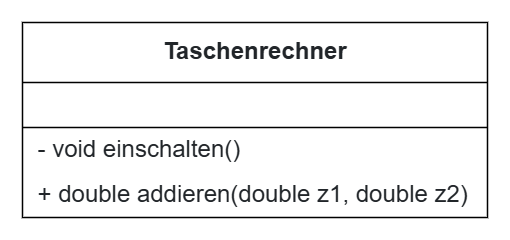
\includegraphics[width=\linewidth]{_Aufgaben//BlocklyJava_Skript//img/H07_KD.png}
}{%
    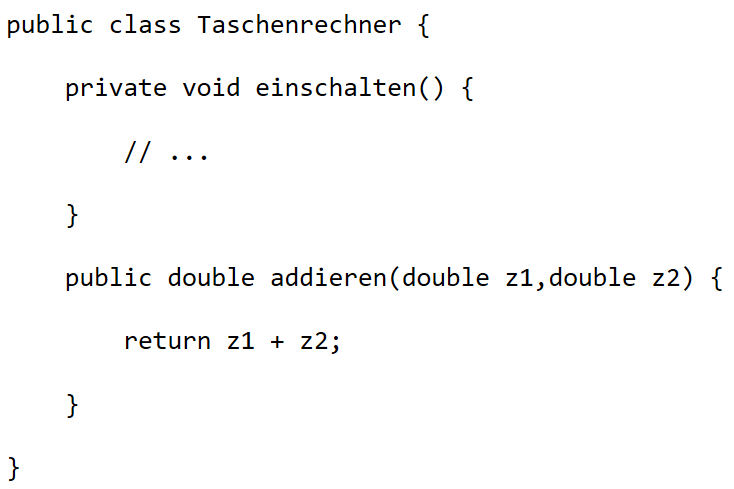
\includegraphics[width=\linewidth]{_Aufgaben//BlocklyJava_Skript//img/H07_Code.png}
}
}


        \Aufgabe{Attribute im Klassendiagramm}{

Findet heraus, wie Attrbiute im Klassendiagramm dargestellt werden. Achtet auf \emphColB{Zugriffsmodifizierer, Datentyp und Name}. Macht eine Skizze auf einem Schmierblatt.

}

        \Hefteintrag{2}{Attribute im Klassendiagramm}{%
Attribute werden im Klassendiagramm folgendermaßen dargestellt:

\centering
\vspace{1cm}
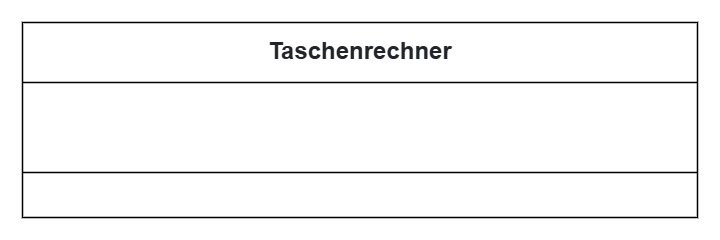
\includegraphics[width=0.7\textwidth]{_Aufgaben/BlocklyJava_Skript/img/H08_KD.png}


\vspace{1cm}

}

        
\begin{minipage}[t]{\textwidth}
\Aufgabe{Struktogramme und Klassendiagramme}

\textbf{Setze folgende Diagramme in BlueJ-Blockly um und notiere den Programmcode auf der nächsten Seite}

\vspace{0.5cm}

\doppelseite{0.45}{0.5}{t}{%
\textbf{Klassendiagramm:}

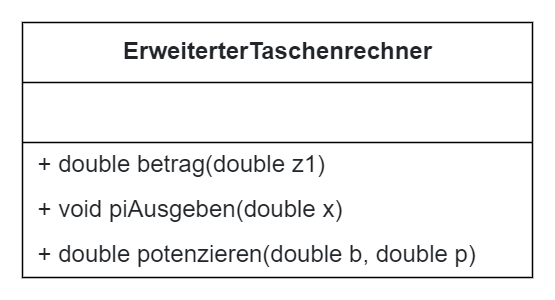
\includegraphics[width=\linewidth]{_Aufgaben/BlocksAndJava/img/klasse.png} 
}{%

\textbf{Struktogramm für piAusgeben(double x):}

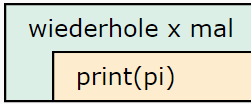
\includegraphics[width=0.6\linewidth]{_Aufgaben/BlocksAndJava/img/strukt_10pi.png}
}

\vspace{1cm}

\textbf{Zeichne hier die Struktogramme für die restlichen Methoden:}

\LoesungKaro{\\
\Large
+ double betrag(double z1) \\
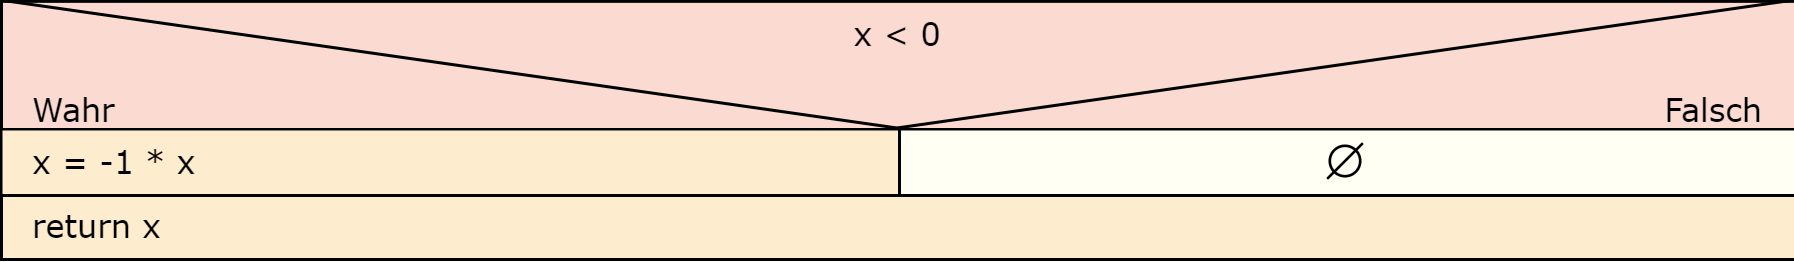
\includegraphics[width=\textwidth]{_Aufgaben/BlocksAndJava/img/strukt_betrag.png} \\\\
+ double potenzieren(double b, double p) \\
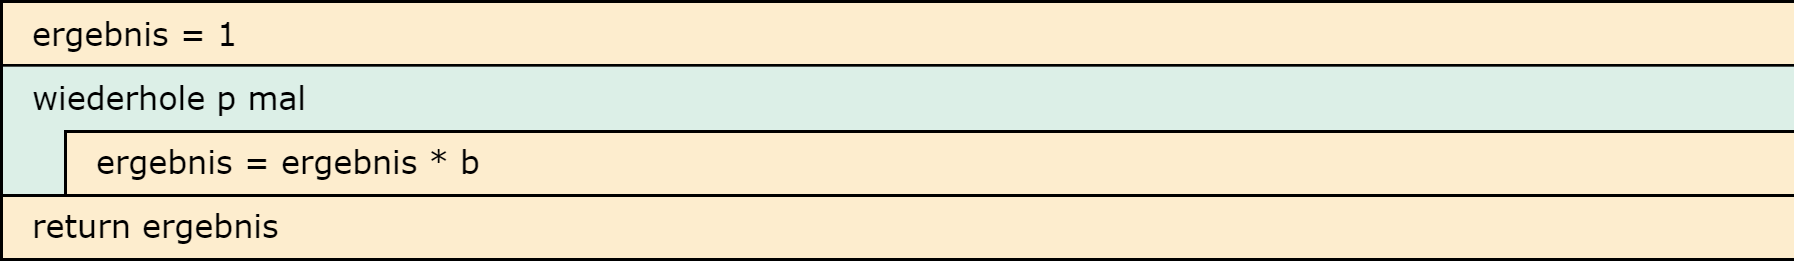
\includegraphics[width=\textwidth]{_Aufgaben/BlocksAndJava/img/strukt_protenz.png}}{25}

    
\end{minipage}


\begin{minipage}[t]{\textwidth}
\Large
\begin{lstlisting}[escapechar=\&]
public class ErweiterterTaschenrechner
{    
    public & \LoesungLuecke{double betrag(double z1) \{ }{15cm} &
    
        & \LoesungLuecke{if(z1 < 0) \{ }{15cm} &
        
            & \LoesungLuecke{z1 = -1 * z1;}{15cm} &
            
        & \LoesungLuecke{\}}{15cm} &   
        
        & \LoesungLuecke{return z1;}{15cm} &   
    }
    public & \LoesungLuecke{void piAusgeben(double x) \{ }{15cm} &
    
        & \LoesungLuecke{for(int i=0; i < x; i++) \{ }{15cm} &
        
            & \LoesungLuecke{System.out.println(Math.PI);}{15cm} &
            
        & \LoesungLuecke{\}}{15cm} &
    }
    public & \LoesungLuecke{double potenzieren(double b, double p) \{ }{15cm} &

        & \LoesungLuecke{double ergebnis = 1.0;}{15cm} &
    
        & \LoesungLuecke{for(int i=0; i < p; i++) \{ }{15cm} &
        
            & \LoesungLuecke{ergebnis = ergebnis * b;}{15cm} &
            
        & \LoesungLuecke{\}}{15cm} &
            
        & \LoesungLuecke{return ergebnis;}{15cm} &
    }
}
\end{lstlisting}

\end{minipage}
        
    }
}